% Provenance (never printed): the national-accounts strand of ../economics_series.md (grade 8: value added, GDP as
% production = income = spending, GDP per person, what it leaves out). Brief: sources/book1/BRIEFS.md, g8-02. Chart
% data: figdata/grade-8/02-gdp (WDI GDP at PPP 2024; Brenland accounts 2025). Ledger: g8:sna-2008,
% g8:sna-household-services.
\chapter{Measuring an Economy: GDP}\label{ch:g8:gdp}

\begin{openingchart}{The ten largest economies in 2024: GDP in total (left, trillions) and per
person (right, thousands), in international dollars of 2021 at purchasing-power parity.}{World
Bank, World Development Indicators, NY.GDP.MKTP.PP.KD and NY.GDP.PCAP.PP.KD, 2024}
\begin{tikzpicture}
\begin{axis}[omrecord, name=tot, xbar, bar width=6pt, xmin=0, xmax=40, ytick=data,
  yticklabels from table={figdata/grade-8/02-gdp/out/largest.csv}{label},
  y tick label style={font=\scriptsize}, xlabel={GDP (trillions)}, width=0.42\linewidth,
  height=0.5\linewidth, enlarge y limits=0.07, nodes near coords,
  nodes near coords align={horizontal}, every node near coord/.append style={font=\tiny}]
\addplot[fill=omDef, draw=none] table[x=total, y=pos] {figdata/grade-8/02-gdp/out/largest.csv};
\end{axis}
\begin{axis}[omrecord, at={(tot.east)}, anchor=west, xshift=0.6cm, xbar, bar width=6pt, xmin=0,
  xmax=90, ytick=data, yticklabels={}, xlabel={GDP per person (thousands)},
  width=0.42\linewidth, height=0.5\linewidth, enlarge y limits=0.07, nodes near coords,
  nodes near coords align={horizontal}, every node near coord/.append style={font=\tiny}]
\addplot[fill=omThm, draw=none] table[x=per_person, y=pos] {figdata/grade-8/02-gdp/out/largest.csv};
\end{axis}
\end{tikzpicture}
\end{openingchart}

% figdata: largest (CHN 33.6 / 23.8; USA 25.7 / 75.7; IND 13.7 / 9.4; GBR 3.7 / 53.4); facts (world_total 174.2,
% top10_share 60.8)
China produced the most in 2024: $33.6$ trillion dollars of goods and services, measured at
the same \omterm{def:g7:money:price}{prices} in every country. The United States came second with $25.7$ trillion, India
third with $13.7$ trillion. Together, the ten largest economies produced $60.8\,\%$ of the
world's $174.2$ trillion. Per person, the order changes. A person in the United States had
$75.7$ thousand dollars of output, in China $23.8$ thousand, in India $9.4$ thousand. These values,
for 2024 from the World Bank, differ a little from those of
\cref{ch:g8:production-and-productivity}, which are for 2023 from another source: different
sources measure in slightly different ways. China and
India are large because they have many people; the United States, Germany and France because
each person produces a lot.

These numbers add up everything a country produces in a year into one sum. This chapter shows
how that sum is built, why the same total can be reached in three ways, and what it leaves out.

\begin{recall}
A \omterm{def:g7:firms:firm}{firm}'s \omterm{def:g7:firms:revenue}{revenue} is the \omterm{def:g7:money:money}{money} it receives from its sales (\cref{ch:g7:firms}). \omterm{def:g6:living-standards:income-per-person}{Income per
person} is a country's \omterm{def:g7:households:income}{income} divided by its population (\cref{ch:g6:living-standards}).
\end{recall}

\section{From sales to value added}

\begin{definition}[Intermediate good]\label{def:g8:gdp:intermediate-good}
An \emph{intermediate good}\index{intermediate good} is a good or service bought by a \omterm{def:g7:firms:firm}{firm} and
used up in producing another good in the same period: flour for a baker, energy for a factory.
\end{definition}

\begin{definition}[Final good]\label{def:g8:gdp:final-good}
A \emph{final good}\index{final good} is a good or service bought by its last user: a \omterm{def:g7:households:household}{household},
the government, a \omterm{def:g7:firms:firm}{firm} buying a machine it will use for years, or a buyer abroad.
\end{definition}

\begin{definition}[Value added]\label{def:g8:gdp:value-added}
The \emph{value added}\index{value added} of a \omterm{def:g7:firms:firm}{firm} in a period is the value of what it sells,
minus the value of the \omterm{def:g8:gdp:intermediate-good}{intermediate goods} it bought:
\[
\text{value added} = \text{sales} - \text{intermediate goods}.
\]
\end{definition}

\begin{omfigure}
\begin{tikzpicture}[econ, x=1cm, y=1cm,
  firm/.style={draw, rounded corners=2pt, fill=black!6, font=\scriptsize, minimum width=2.2cm,
    minimum height=0.9cm, align=center},
  va/.style={fill=omDef!35, draw=none}, inter/.style={fill=black!15, draw=none}]
  \node[firm] (f) at (0,4.4) {farm\\sells wheat: 300};
  \node[firm] (m) at (3.8,4.4) {mill\\sells flour: 500};
  \node[firm] (b) at (7.6,4.4) {bakery\\sells bread: 900};
  \draw[-{Stealth}] (f) -- node[above, font=\scriptsize] {wheat} (m);
  \draw[-{Stealth}] (m) -- node[above, font=\scriptsize] {flour} (b);
  % bars: 1 cm = 300 dalens
  \fill[va] (-0.5,0) rectangle (0.5,1);
  \fill[inter] (3.3,0) rectangle (4.3,1);
  \fill[va] (3.3,1) rectangle (4.3,1.667);
  \fill[inter] (7.1,0) rectangle (8.1,1.667);
  \fill[va] (7.1,1.667) rectangle (8.1,3);
  \node[font=\scriptsize, above] at (0,1) {300};
  \node[font=\scriptsize, above] at (3.8,1.667) {200};
  \node[font=\scriptsize, above] at (7.6,3.0) {400};
  \node[font=\scriptsize] at (3.8,0.5) {300};
  \node[font=\scriptsize] at (7.6,0.83) {500};
  \draw (-1,0) -- (8.6,0);
  \fill[va] (9.0,2.3) rectangle (9.3,2.6); \node[font=\scriptsize, right] at (9.3,2.45) {value added};
  \fill[inter] (9.0,1.8) rectangle (9.3,2.1); \node[font=\scriptsize, right] at (9.3,1.95) {bought from};
  \node[font=\scriptsize, right] at (9.3,1.6) {the firm before};
\end{tikzpicture}

{\small A chain of three \omterm{def:g7:firms:firm}{firms}, in dalens. Each bar is a \omterm{def:g7:firms:firm}{firm}'s sales; the grey part is what it
bought from the \omterm{def:g7:firms:firm}{firm} before, the blue part its \omterm{def:g8:gdp:value-added}{value added}. The \omterm{def:g8:gdp:value-added}{value added}, $300 + 200 + 400 =
900$, equals the \omterm{def:g7:money:price}{price} of the bread.}
\end{omfigure}

Adding the three \omterm{def:g7:firms:firm}{firms}' sales gives $300 + 500 + 900 = 1\,700$ dalens, but only 900 dalens of
bread were produced for someone to eat: the wheat is counted in the flour, and the flour in the
bread. Adding sales counts the same wheat three times. Adding \omterm{def:g8:gdp:value-added}{value added} counts each step once.

\begin{omfigure}
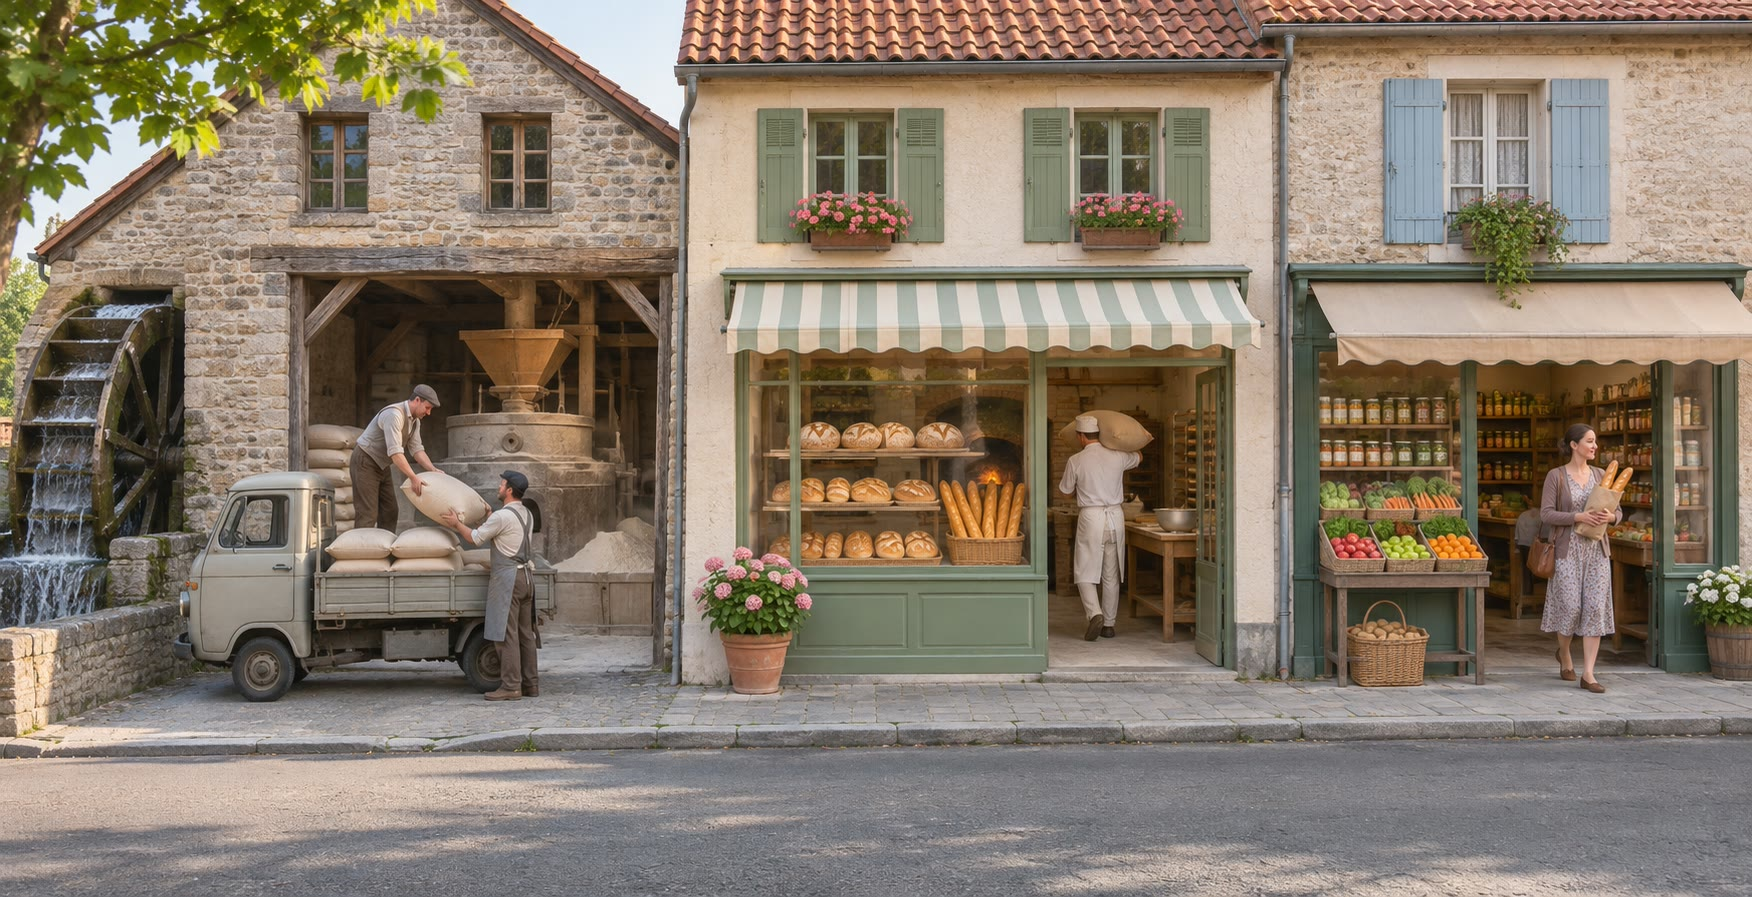
\includegraphics[width=0.52\linewidth]{images/book1/ai/g8-gdp-mill-bakery-shop.jpg}

{\small A mill, a bakery and a shop in one street. Each adds value to what it buys from the one
before.}
\end{omfigure}

\section{Gross domestic product}

\begin{definition}[Gross domestic product]\label{def:g8:gdp:gdp}
The \emph{gross domestic product}\index{gross domestic product (GDP)} (GDP) of a country in a year
is the value of all \omterm{def:g8:gdp:final-good}{final goods} and services produced in the country in that year; equivalently,
the sum of the \omterm{def:g8:gdp:value-added}{value added} of all its producers.
\end{definition}

``Domestic'' means produced inside the country, by anyone. ``Gross'' means that the machines and
buildings worn out during the year are not subtracted.

\begin{measure}[How GDP is measured]
% ledger: g8:sna-household-services
National statistics offices follow a common manual, the System of National Accounts, written
together by the United Nations and other international organisations. Offices combine tax records, surveys of \omterm{def:g7:firms:firm}{firms} and \omterm{def:g7:households:household}{households}, and the accounts of the
government. Some values must be estimated: the rent that owners would pay for the homes they live
in is counted, as if they rented them to themselves; the services that members of a \omterm{def:g7:households:household}{household}
produce for each other, such as cooking and cleaning, are left out by rule. In many countries, first
estimates are published a few weeks after a quarter ends and revised for years as more data arrive.
\end{measure}

\begin{dated}{2026}
% ledger: g8:sna-2008, g8:sna-2025-adopted, g8:sna-2025-window
Most countries still compile their accounts by the 2008 edition of the manual, which the statistical
commission of the United Nations adopted unanimously as the international standard. In March 2025
the same commission adopted a revised edition, the 2025 System of National Accounts. Countries are
asked to move to it by 2029 or 2030.
\end{dated}

\section{Three ways to the same total}

Every dalen spent on a \omterm{def:g8:gdp:final-good}{final good} is received by someone. The baker's 900 dalens pay the
farmer's and the miller's \omterm{def:g7:households:wage}{wages} and \omterm{def:g7:firms:profit}{profits}, and the baker's own. So the same total can be
reached in three ways:
\begin{itemize}
  \item \emph{production}: add the \omterm{def:g8:gdp:value-added}{value added} of all producers;
  \item \emph{\omterm{def:g7:households:income}{income}}: add all \omterm{def:g7:households:wage}{wages}, \omterm{def:g7:firms:profit}{profits}, rents and interest earned in production;
  \item \emph{spending}: add all spending on \omterm{def:g8:gdp:final-good}{final goods}: by \omterm{def:g7:households:household}{households} ($C$, consumption), by
        \omterm{def:g7:firms:firm}{firms} on new machines and buildings ($I$, investment), by the government ($G$), and by
        buyers abroad ($X$, \omterm{def:g6:a-connected-world:export}{exports}), minus what is bought from abroad ($M$, \omterm{def:g6:a-connected-world:import}{imports}):
\end{itemize}
\[
\text{GDP} = C + I + G + X - M.
\]
\omterm{def:g6:a-connected-world:import}{Imports} are subtracted because they are included in $C$, $I$ and $G$ but were produced in another
country.

\begin{omfigure}
\begin{tikzpicture}[econ, x=1cm, y=1cm,
  agent/.style={draw, rounded corners=3pt, very thick, minimum width=2.6cm, minimum height=1.3cm,
    align=center, font=\small}]
  \node[agent, fill=omDef!12] (h) at (0,0) {households};
  \node[agent, fill=omThm!10] (f) at (7,0) {firms};
  \draw[-{Stealth}, very thick, omDef] (h.north east) to[bend left=22]
    node[below, font=\scriptsize, text=black, align=center] {spending on\\goods and services} (f.north west);
  \draw[-{Stealth}, very thick, omThm] (f.south west) to[bend left=22]
    node[above, font=\scriptsize, text=black, align=center] {incomes: wages, profits,\\rents, interest} (h.south east);
  \draw[-{Stealth}, thick, black!60, dashed] (f.north) to[bend right=55]
    node[above, font=\scriptsize, text=black] {goods and services} (h.north);
  \draw[-{Stealth}, thick, black!60, dashed] (h.south) to[bend right=55]
    node[below, font=\scriptsize, text=black] {work, capital, land} (f.south);
\end{tikzpicture}

{\small The circular flow, simplified to \omterm{def:g7:households:household}{households} and \omterm{def:g7:firms:firm}{firms}. \omterm{def:g7:money:money}{Money} flows one way (solid
arrows); goods, services and work flow the other way (dashed). Spending by \omterm{def:g7:households:household}{households} is \omterm{def:g7:households:income}{income}
of \omterm{def:g7:firms:firm}{firms}, which pay it out as \omterm{def:g7:households:income}{incomes} to \omterm{def:g7:households:household}{households}.}
\end{omfigure}

\begin{omchart}{Brenland's GDP by spending, 2025, in billions of dalens: consumption, investment,
government spending and exports add up; imports are subtracted (invented data).}{Brenland
national accounts (the series' invented country)}
\begin{tikzpicture}
\begin{axis}[omrecord, xbar, bar width=8pt, xmin=-240, xmax=460, ytick=data,
  yticklabels from table={figdata/grade-8/02-gdp/out/brenland_spending.csv}{item},
  y tick label style={font=\scriptsize}, xlabel={Billions of dalens}, width=0.7\linewidth,
  height=0.45\linewidth, enlarge y limits=0.1, nodes near coords,
  every node near coord/.append style={font=\scriptsize}]
\addplot[fill=omDef, draw=none] table[x=value, y=pos] {figdata/grade-8/02-gdp/out/brenland_spending.csv};
\end{axis}
\end{tikzpicture}
\end{omchart}

\section{GDP per person}

\begin{definition}[GDP per person]\label{def:g8:gdp:gdp-per-person}
\emph{GDP per person}\index{GDP per person} is a country's GDP divided by its population.
\end{definition}

% figdata: facts (gdp 393264 millions, pop 9291 thousands, gdp_per_person 42327)
Brenland's GDP in 2025 was $393\,264$ million dalens, and it had $9\,291$ thousand people. Its \omterm{def:g8:gdp:gdp-per-person}{GDP
per person} was
\[
393\,264\,000\,000 \div 9\,291\,000 \approx 42\,327 \text{ dalens}.
\]
To compare countries, GDP is converted into one currency. The opening chart uses
purchasing-power parity: the same goods are valued at the same \omterm{def:g7:money:price}{prices} everywhere, so that a
dollar of GDP buys the same in every country (\cref{ch:g9:exchange-rates-and-purchasing-power}).

\section{What GDP leaves out}

\begin{measure}[What GDP leaves out]
GDP counts what is sold or could be sold. It leaves out the cooking, cleaning and caring done
by members of a \omterm{def:g7:households:household}{household} for each other; the value of free time; the harm done to air, water
and climate, and the wearing out of nature; and how the \omterm{def:g7:households:income}{income} is shared among people. A country
where people work longer hours for the same output has the same GDP as one where they work
less. GDP was built to measure production, not wellbeing; it is used as a guide to \omterm{def:g6:living-standards:living-standard}{living
standards} because, across countries, it goes together with health, schooling and life
expectancy (\cref{ch:g6:health-and-population}).
\end{measure}

\section{Exercises}

\begin{exercise}[$\star$]\label{exo:g8:gdp:1}
Use the opening chart. Which economy was the largest in total in 2024? Which of the ten had the
highest \omterm{def:g8:gdp:gdp-per-person}{GDP per person}?
\end{exercise}

\begin{exercise}[$\star$]\label{exo:g8:gdp:2}
A farmer sells cotton for 200 dalens to a spinner, who sells yarn for 350 dalens to a weaver, who
sells cloth for 600 dalens to \omterm{def:g7:households:household}{households}. Compute each \omterm{def:g7:firms:firm}{firm}'s \omterm{def:g8:gdp:value-added}{value added}, and their sum.
\end{exercise}

\begin{exercise}[$\star$]\label{exo:g8:gdp:3}
In a small island economy in a year, \omterm{def:g7:households:household}{households} buy bread for 900 and fish for 400; a fisher buys
a new boat for 300; the baker buys flour for 500. All are in dalens and produced on the island.
What is the island's GDP?
\end{exercise}

\begin{exercise}[$\star$]\label{exo:g8:gdp:4}
Use the opening chart. Among the ten, which had the lowest \omterm{def:g8:gdp:gdp-per-person}{GDP per person}?
\end{exercise}

\begin{exercise}[$\star\star$]\label{exo:g8:gdp:5}
In exercise 2, a clerk adds up all the sales. What total does the clerk find? By how much does it
overstate the value of what was produced?
\end{exercise}

\begin{exercise}[$\star\star$]\label{exo:g8:gdp:6}
Kestria's GDP is $120\,000$ million kests and its population 4 million. Compute its \omterm{def:g8:gdp:gdp-per-person}{GDP per person}.
\end{exercise}

\begin{exercise}[$\star\star$]\label{exo:g8:gdp:7}
In 2025, Brenland's consumption was $225\,014$, investment $88\,484$, government spending
$78\,653$, \omterm{def:g6:a-connected-world:export}{exports} $129\,777$ and \omterm{def:g6:a-connected-world:import}{imports} $128\,664$, in millions of dalens. Compute its GDP.
\end{exercise}

\begin{exercise}[$\star\star$]\label{exo:g8:gdp:8}
Use the opening chart. How many times larger was China's GDP than that of the United States? How
many times larger was \omterm{def:g8:gdp:gdp-per-person}{GDP per person} in the United States than in China?
\end{exercise}

\begin{exercise}[$\star\star$]\label{exo:g8:gdp:9}
Describe what you would need to observe to conclude that \omterm{def:g8:gdp:gdp-per-person}{GDP per person} is a poor guide to how
well people live in a country.
\end{exercise}

\begin{exercise}[$\star\star\star$]\label{exo:g8:gdp:10}
A family buys 12 dalens of food and cooks dinner at home. The next week, it eats the same dinner at
a restaurant for 40 dalens; the restaurant bought the same 12 dalens of food. (a) How much does
each dinner add to GDP? (b) Did the family's wellbeing change by as much?
\end{exercise}

\begin{exercise}[$\star\star\star$]\label{exo:g8:gdp:11}
An economy has two \omterm{def:g7:firms:firm}{firms}. A farm sells wheat for 300 dalens to a bakery; it pays 200 in \omterm{def:g7:households:wage}{wages} and
keeps 100 as \omterm{def:g7:firms:profit}{profit}. The bakery sells bread for 900 dalens to \omterm{def:g7:households:household}{households}; it pays 300 for wheat,
450 in \omterm{def:g7:households:wage}{wages} and keeps 150 as \omterm{def:g7:firms:profit}{profit}. Compute GDP (a) by \omterm{def:g8:gdp:value-added}{value added}, (b) by \omterm{def:g7:households:income}{incomes}, (c) by
spending.
\end{exercise}

\begin{exercise}[$\star\star\star$]\label{exo:g8:gdp:12}
Two countries have the same \omterm{def:g8:gdp:gdp-per-person}{GDP per person}. Name two things about who receives the \omterm{def:g7:households:income}{income} that \omterm{def:g8:gdp:gdp-per-person}{GDP
per person} cannot tell, and say what data would tell one of them.
\end{exercise}

\section{Problem: Brenland's Accounts}

\begin{problem}[{Weekend problem --- value added along a chain of Brenland firms, GDP from
spending, and GDP per person}]
\label{pb:g8:gdp:1}
Everything in this problem is invented.

\medskip
\noindent\textbf{Part I --- A chain of firms.} In a year, a Brenland orchard sells apples for 40
million dalens to a juice \omterm{def:g7:firms:firm}{firm}. A glass works sells bottles for 20 million dalens to the same juice
\omterm{def:g7:firms:firm}{firm}, from sand it digs itself. The juice \omterm{def:g7:firms:firm}{firm} sells its juice for 90 million dalens to shops,
which sell it to \omterm{def:g7:households:household}{households} for 150 million dalens.
\begin{enumerate}
  \item What is the \omterm{def:g8:gdp:value-added}{value added} of the orchard and of the glass works?
  \item What is the \omterm{def:g8:gdp:value-added}{value added} of the juice \omterm{def:g7:firms:firm}{firm}?
  \item What is the \omterm{def:g8:gdp:value-added}{value added} of the shops?
  \item Add the four values added. Compare with the \omterm{def:g7:households:household}{households}' spending on juice.
\end{enumerate}

\medskip
\noindent\textbf{Part II --- The spending side.} In 2025, Brenland's accounts give, in millions of
dalens: consumption $225\,014$, investment $88\,484$, government spending $78\,653$, \omterm{def:g6:a-connected-world:export}{exports}
$129\,777$, \omterm{def:g6:a-connected-world:import}{imports} $128\,664$.
\begin{enumerate}[resume]
  \item Compute Brenland's GDP.
  \item Compute its net \omterm{def:g6:a-connected-world:export}{exports}, $X - M$.
  \item Explain why \omterm{def:g6:a-connected-world:import}{imports} are subtracted.
  \item Which spending item is the largest?
\end{enumerate}

\medskip
\noindent\textbf{Part III --- Per person.} Brenland had $9\,291$ thousand people in 2025. In
2024, its GDP was $379\,562$ million dalens and its population $9\,235$ thousand.
\begin{enumerate}[resume]
  \item Compute the shares of consumption, investment and government spending in GDP in 2025, in
        percent, to one decimal.
  \item Compute \omterm{def:g8:gdp:gdp-per-person}{GDP per person} in 2024, to the nearest dalen.
  \item Compute \omterm{def:g8:gdp:gdp-per-person}{GDP per person} in 2025, to the nearest dalen.
  \item Compute the \omterm{def:g6:reading-economic-charts:rate-of-change}{rate of change} of \omterm{def:g8:gdp:gdp-per-person}{GDP per person} from 2024 to 2025, in percent. \omterm{def:g7:money:price}{Prices} in
        Brenland rose by about $1.7\,\%$ in that year: did the quantity of goods per person rise by
        as much as \omterm{def:g8:gdp:gdp-per-person}{GDP per person}?
\end{enumerate}
\end{problem}
